\documentclass{article}
\usepackage{geometry}
 \geometry{
 a4paper,
 total={170mm,270mm},
 left=20mm,
 top=10mm,
 }
\usepackage{float}
\usepackage{graphicx}
\usepackage{subcaption}
\usepackage{enumitem}
\usepackage{caption}
\usepackage{amsmath}
\newcommand*{\addheight}[2][.5ex]{%
  \raisebox{0pt}[\dimexpr\height+(#1)\relax]{#2}%
}
\title{\textbf{Chaotic Dynamics - CSCI 5446} \\
Problem Set 6}
\author{Santhanakrishnan Ramani}
\begin{document}
\maketitle

\section*{Problem 1}
\begin{enumerate}[label=(\alph*)]

\item 
The Figure \ref{fig:prob1a} represents the temporal Poincare section of the pendulum trajectory emanating from the point $[\theta,\omega] = [0.01,0]$ with $m = 0.1kg, l = 0.1m, \beta = 0 \,\,and\,\, \alpha = A = 0$ on the surface of section $\sum :t = nT_{0}$, where $T_{0} = 0.6347$ being the natural period of the device. \par\medskip
\begin{minipage}{\linewidth}
{
\centering 
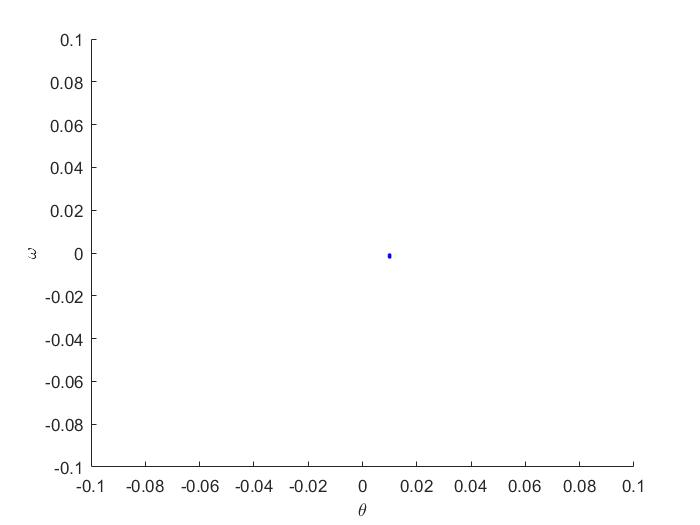
\includegraphics[scale=0.4]{images/prob1a.jpg}
\captionof{figure}{Temporal Poincare Section}
\label{fig:prob1a}
}
\par\medskip
Yes, this is what is expected. Since, the trajectory is sampled at it's natural period it is expected that there is only a single point in the section. But due to the numerical error that arises by using rk4 the points are closely clustered nearby to its starting point, making the point distorted.
\end{minipage}

\item
The Figure \ref{fig:prob1b} represents the temporal Poincare section of the pendulum with parameters same as prob1a, but by choosing a $T = 0.75$ not rationally related to $T_{0} = 0.6347$ \par\medskip
\begin{minipage}{\linewidth}
{
\centering 
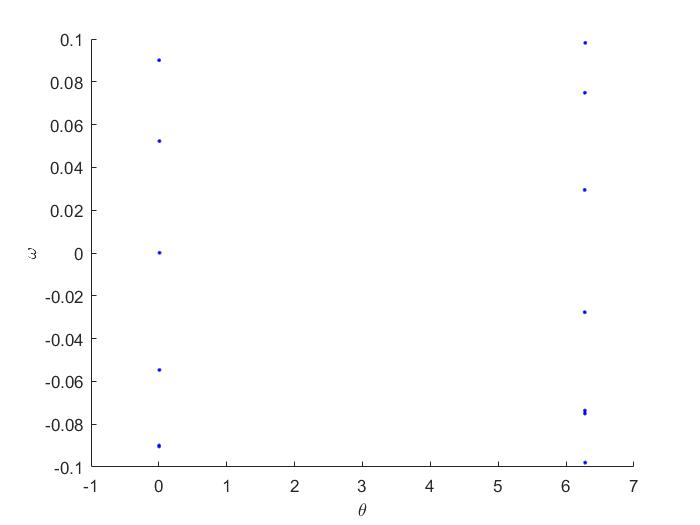
\includegraphics[scale=0.4]{images/prob1b.jpg}
\captionof{figure}{Temporal Poincare Section}
\label{fig:prob1b}
}
\end{minipage}
\par\medskip

The difference between the plots in prob1a and prob1b is that, in the latter we see points lying on two sides of the plots, meaning the points below and above the initial condition are sampled at different instant of time, which wasn't the case in the former.

\item
The Figure \ref{fig:prob1c} represents the temporal Poincare section of the pendulum with chaotic trajectory  emanating from the point $[\theta,\omega] = [0.01,0]$ with $m = 0.1kg, l = 0.1m, \beta = 0.25, \alpha = 7.4246 \,\,and\,\, A = 1.1$ on the surface of section $\sum :t = nT_{Drive}$, where $T_{Drive} = 0.8463$  \par\medskip
\begin{minipage}{\linewidth}
{
\centering 
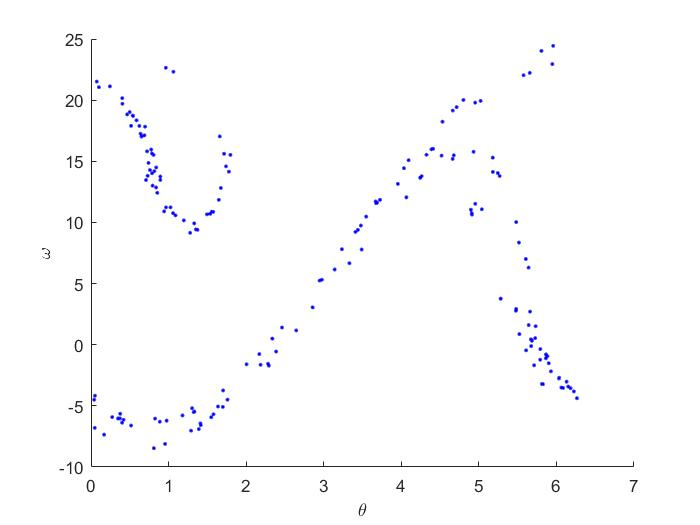
\includegraphics[scale=0.4]{images/prob1c.jpg}
\captionof{figure}{Temporal Poincare Section}
\label{fig:prob1c}
}
\end{minipage}

\item
On increasing the time step keeping the time span covered by the trajectory constant, we see the shape of the plot obtained remains nearly the same, but the number of points being plotted increases as time step increases. The reason being as the time step is increased, the length of trajectory it covers increases, and it pierces the respective sections faster.  

\end{enumerate}

\section*{Problem 2}
\begin{enumerate}[label=(\alph*)]

\item
As we could see from the figure below there isn't a big difference that could be noted when the chaotic trajectory of the pendulum plotted on to a poincare section by using interpolation compared to the one in prob1c.\par\medskip
\begin{minipage}{\linewidth}
{
\begin{table}[H]
\centering
\begin{tabular}{|c|c|}
	\hline
	\addheight{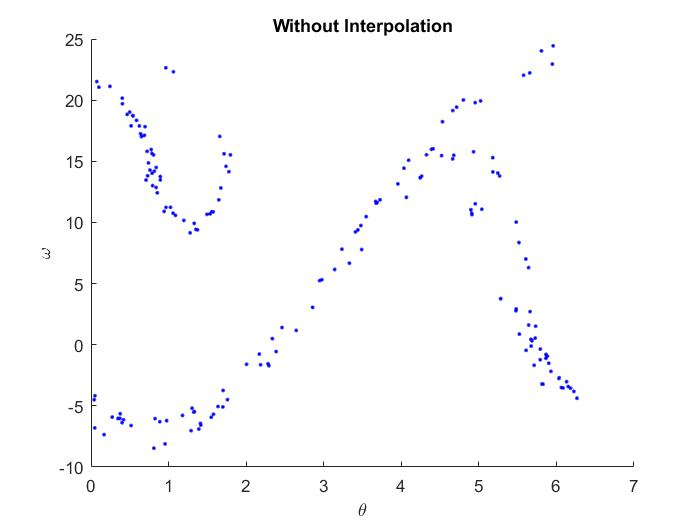
\includegraphics[height=75mm,width=75mm]{images/prob2a.jpg}} &
    \addheight{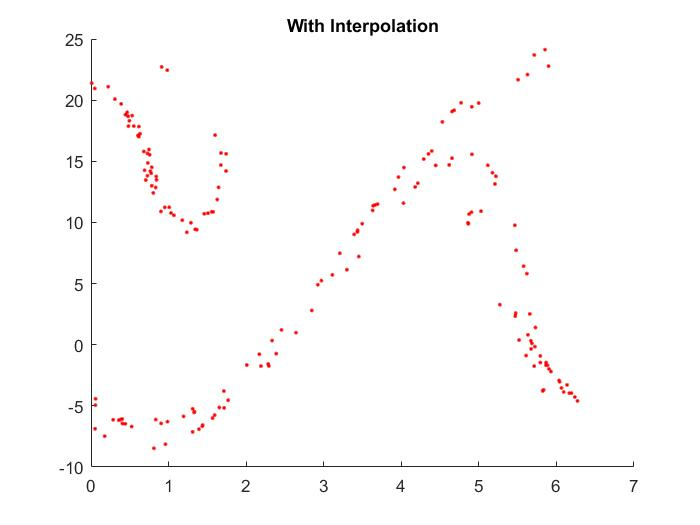
\includegraphics[height=75mm,width=75mm]{images/prob2b.jpg}} \\
    \hline
\end{tabular}
\end{table}
}
\end{minipage}
\par\medskip
Below figure shows us the effect of increasing the time step. It appears to have the same effect as explained in prob1d, the basic structure of the plot remains the same but the plot becomes dense as number of pointed plotted increases as time step increases.
\par\medskip
\begin{minipage}{\linewidth}
{
\begin{table}[H]
\centering
\begin{tabular}{|c|c|}
	\hline
	\addheight{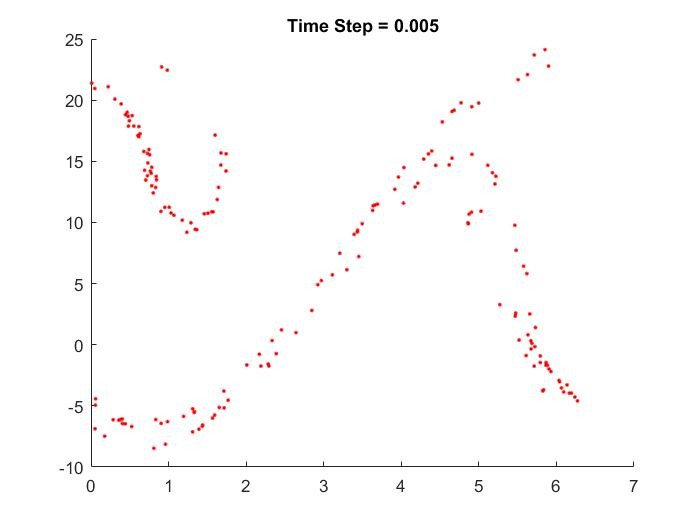
\includegraphics[width=75mm]{images/prob2d1.jpg}} &
    \addheight{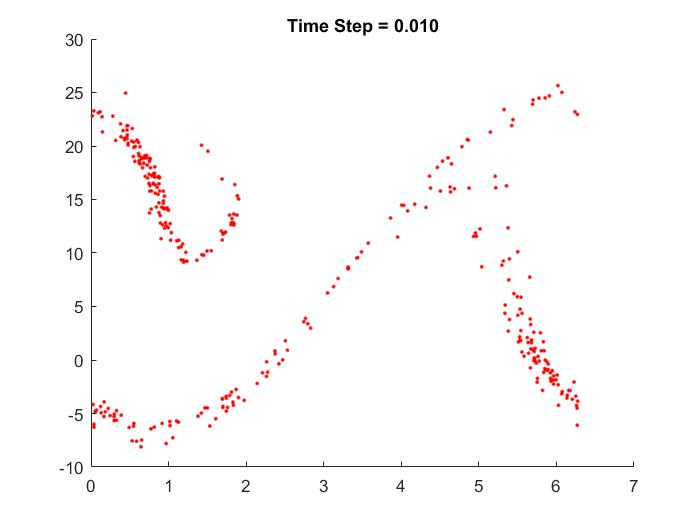
\includegraphics[width=75mm]{images/prob2d2.jpg}} \\
    \hline
    \addheight{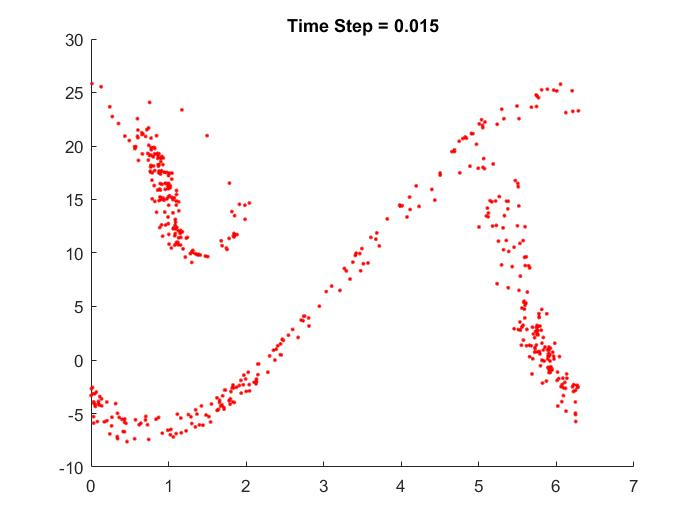
\includegraphics[width=75mm]{images/prob2d3.jpg}} &
    \addheight{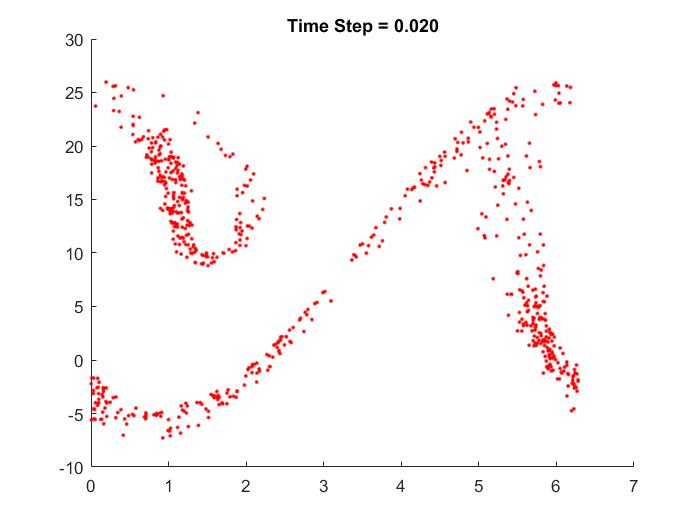
\includegraphics[width=75mm]{images/prob2d4.jpg}} \\
    \hline
\end{tabular}
\end{table}
}
\end{minipage}

\end{enumerate}

\section*{Problem 3}
The Figures \ref{fig:prob3a} and \ref{fig:prob3b} represent the spatial poincare section of the Lorenz attractor with $r=50$ on the planes $y=20 \,\&\, y=2x$ repectively\par\medskip
\begin{figure}[H]
\centering 
\begin{subfigure}{.5\textwidth}
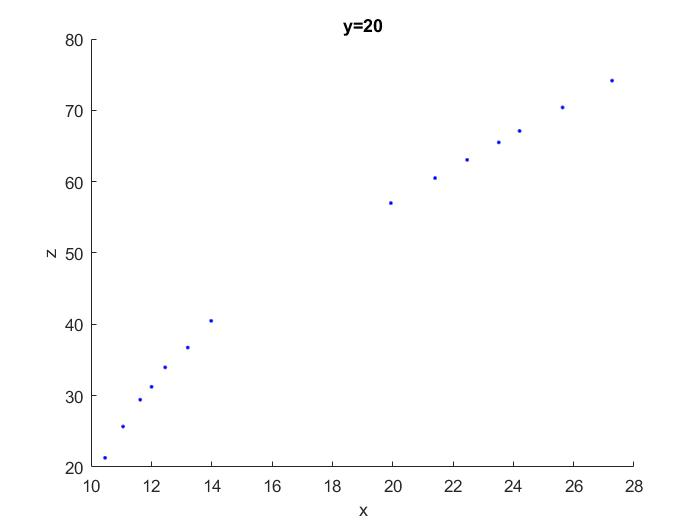
\includegraphics[width=90mm]{images/prob3a.jpg}
\captionof{figure}{spatial Poincare Section}
\label{fig:prob3a}
\end{subfigure}%
\begin{subfigure}{.5\textwidth}
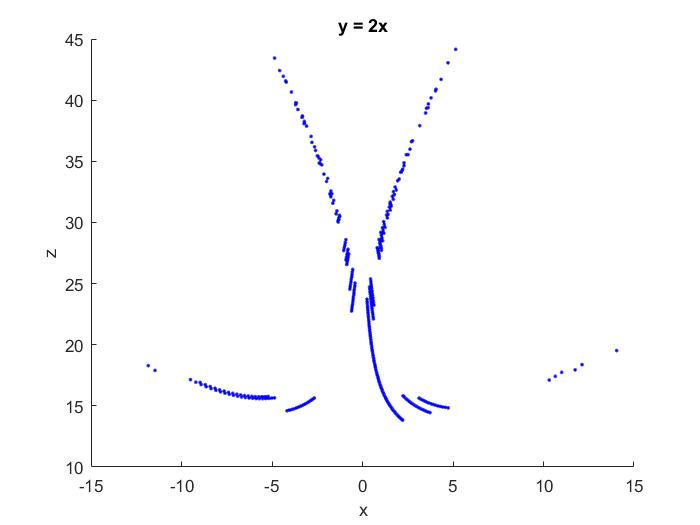
\includegraphics[width=90mm]{images/prob3b.jpg}
\captionof{figure}{spatial Poincare Section}
\label{fig:prob3b}
\end{subfigure}
\end{figure}

\end{document}
